\documentclass[conference]{IEEEtran}
%\IEEEoverridecommandlockouts % needed to identify funding in the first footnote. If unneeded, comment it.
\usepackage{cite}
\usepackage{amsmath,amssymb,amsfonts, gensymb}
\usepackage{algorithmic}
\usepackage{graphicx}
\usepackage{textcomp}
\usepackage{hyperref}
\usepackage{xcolor}
\usepackage{lipsum}
\usepackage{stfloats} % elimina la restricción de LaTeX de un solo float [b] por columna.
\usepackage{caption}
\usepackage{tikz}
\usepackage{circuitikz}
\usepackage{comment}
\usepackage{balance}

\usepackage{colortbl}
\definecolor{coppercolor}{RGB}{229, 179, 58}
\definecolor{dielectriccolor}{RGB}{112, 173, 104}

\def\BibTeX{{\rm B\kern-.05em{\sc i\kern-.025em b}\kern-.08em
    T\kern-.1667em\lower.7ex\hbox{E}\kern-.125emX}}
\begin{document}

% ========================= TITLE =========================
\title{Design and Characterization of a GaN Class AB S-Band Power Amplifier for CubeSat Downlink Applications\\

%\thanks{Identify applicable funding agency here. If none, delete this.}
}


\begin{comment}
% ========================= AUTHORS =========================
\author{
    \IEEEauthorblockN{
        Facundo Repetto\IEEEauthorrefmark{1},
        Liam Duggan\IEEEauthorrefmark{1},
        Manuel G. Redondo\IEEEauthorrefmark{2},
        Sebastián Verrastro\IEEEauthorrefmark{1},
        Lucas Liaño\IEEEauthorrefmark{1},
    }
    \IEEEauthorblockA{
        \IEEEauthorrefmark{1}Grupo de Inteligencia Artificial y Robótica,
        Univ. Tecnológica Nacional--FRBA, Buenos Aires, Argentina \\
        facurepe@frba.utn.edu.ar,  lduggan@frba.utn.edu.ar
        %\{facurepe, lduggan\}@frba.utn.edu.ar
    }
    \IEEEauthorblockA{
        \IEEEauthorrefmark{2} Instituto de Tecnologías en Detección y Astropartículas, Gral. San Martín, Argentina
    }
}
\end{comment}

\maketitle

% ========================= ABSTRACT =========================
\begin{abstract}
This work presents the design, simulation, and experimental characterization of a class AB S-band power amplifier (PA) for CubeSat downlink applications in Low Earth orbit (LEO). The amplifier employs a discrete GaN HEMT, selected for its superior power density and thermal performance. A link budget analysis determined that 1 W output power is sufficient for a 2.96 Mbps downlink using QPSK modulation at elevation angles above 20 degrees. The circuit was designed on a four-layer FR4 substrate, with matching networks implemented using distributed components. Load-pull simulations under large-signal harmonic balance analysis were used to determine the optimum load impedance maximizing power-added efficiency (PAE). Measured small-signal characterization shows a center frequency of 2.11 GHz, a gain of 13.26 dB, and a VSWR below 1.92:1 over a 70 MHz bandwidth. Large-signal measurements yield a 1 dB compression point (P1dB) of 30.3 dBm, an OIP3 of 39.83 dBm, and a drain efficiency of 32.94\% at an output power of 30.92 dBm. Strong agreement between simulations and measurements validates the design methodology, positioning this platform as a foundation for future RF developments in small satellite systems.
\end{abstract}

\begin{IEEEkeywords}
Gallium nitride (GaN), power amplifiers, Class AB, CubeSat, S-Band, large signal simulation
\end{IEEEkeywords}

% ========================= SECCIONES =========================
\section{Introduction}
Power amplifiers (PAs) are a critical subsystem in any RF transmitter chain, responsible for boosting the signal to the power levels required for reliable communications over long distances. In satellite systems, this role is particularly demanding, as the PA must deliver sufficient power to close the downlink budget while operating under strict energy, mass, and thermal constraints, and withstanding the harsh conditions of the space environment, including ionizing radiation, wide thermal swings, and high vacuum.

Gallium Nitride High Electron Mobility Transistors (GaN HEMTs) have established themselves as strong competitors to conventional technologies such as GaAs and Si in RF power amplifiers designs, given their superior breakdown voltage, elevated power density, wide thermal operating range, and capability for operation at high frequencies \cite{Boomer2020, Mishra2008, Deblecker2015}. These properties make GaN transistors well suited for a wide range of applications, such as broadband, high-power, and high-efficiency designs.

In parallel, the CubeSat standard has fundamentally changed the landscape of space missions. Originally conceived as a low-cost platform based on 10×10×10\,cm modular units (1\,U) \cite{cubesat_design_spec}, CubeSats have evolved into capable research and commercial platforms used for several applications, such as Earth observation, telecommunications, and technology demonstration. Their reduced size and mass impose severe constraints on the RF subsystems: the PA must be compact, efficient, and capable of sustaining reliable operation in LEO without active thermal management or human intervention.

This work presents the design and experimental characterization of a single-stage, Class AB, 1\,W GaN power amplifier targeting the S-Band downlink at 2.2\,GHz for CubeSat applications. The output power level was determined from a link budget analysis supporting data rates up to 4.44\,Mbps.

Building on well-established techniques (Class AB biasing, load-pull-based matching, resistive stabilization), this work proposes a link-budget-driven, low-cost FR4 design tailored to CubeSat downlinks, validated through full experimental characterization and an analysis of the simulation-to-measurement frequency shift.

This paper is organized as follows. Section~II presents the link budget analysis and theoretical background. Section~III describes the proposed circuit design, Section~IV the measurement setups, and Section~V the experimental results. Section~VI draws conclusions.
\section{Materials and Methods}
\subsection{Link Budget Analysis} \label{sec:link_budget}
Downlink communications from LEO face challenges associated with link geometry and the propagation environment. While orbital altitudes are substantially lower than geostationary systems, free-space path losses remain significant and vary with the elevation angle. Additional impairments include electromagnetic interference from co-existing systems and atmospheric and ionospheric effects that cause signal attenuation and fluctuations. These conditions, combined with the limited transmit power available on CubeSat platforms, impose tight design margins.

A link budget analysis was carried out to determine the minimum elevation angle at which reliable communication is feasible for a fixed channel bandwidth of 2\,MHz, evaluating three modulation schemes: QPSK, 8PSK, and 16PSK. These schemes were selected for their constant or near-constant envelope, which limits amplitude variations in the transmitted signal and reduces the risk of driving the amplifier into its nonlinear region \cite{Cripps2006}. For a roll-off factor of $\alpha = 0.35$, this bandwidth yields symbol rates and achievable data rates of 2.96\,Mbps for QPSK, 4.44\,Mbps for 8PSK, and 5.93\,Mbps for 16PSK. The calculations were performed following the methodology described in \cite{Seybold2005}, implemented in a Python script that allowed parametric tuning of the system parameters. The assumed values are listed in Table~\ref{tab:link_budget_params}.

\begin{table}[b]
    \caption{Link Budget Parameters}
    \label{tab:link_budget_params}
    \centering
    \renewcommand{\arraystretch}{1.15}
    \begin{tabular}{lcc}
        \hline\hline
        \textbf{Parameter} & \textbf{Symbol} & \textbf{Value} \\
        \hline
        Bandwidth               & $BW$               & 2\,MHz   \\
        Transmit power          & $P_T$              & 0\,dBW   \\
        TX antenna gain         & $G_T$              & 7\,dBi   \\
        RX antenna gain         & $G_R$              & 27\,dBi  \\
        Transmitter losses      & $L_{TX}$           & 1\,dB    \\
        Pointing loss           & $L_\text{point}$   & 1\,dB    \\
        Atmospheric losses      & $L_\text{atm}$     & 1\,dB    \\
        Antenna noise temp.     & $T_\text{ant}$     & 55\,K    \\
        LNA noise temp.         & $T_\text{LNA}$     & 70\,K    \\
        Orbital altitude        & $h$                & 600\,km  \\
        \hline\hline
    \end{tabular}
\end{table}

Free-space path loss was computed from the satellite-to-ground distance $D(\epsilon)$, given by \eqref{eq_D}

\begin{equation}
    D = \sqrt{(r_E + h)^2 - r_E^2 \cos^2{\epsilon}} - r_E \sin{\epsilon}
    \label{eq_D}
\end{equation}

where $r_E$ is Earth's mean radius, $h = 600\,\text{km}$ is the orbital altitude, corresponding to the region of highest orbital object density in LEO (600--800\,km)~\cite[Sec.~1.3.1]{AnzMeador2018}, and $\epsilon$ is the elevation angle. For each modulation scheme, a 1\,dB margin above the minimum $E_b/N_0$ required for a bit error rate (BER) of $10^{-5}$ was imposed.

The operating frequency was set to 2.2\,GHz, in proximity to both the 2170--2200\,MHz band allocated to the Mobile Satellite Service (MSS) for downlinks and the 2200--2290\,MHz band designated for space research, as defined by the ITU Radio Regulations~\cite{ITU_RR2024}. Operating near this boundary ensures spectral compatibility with MSS systems while remaining aligned with frequencies used in space exploration and research missions.

Fig.~\ref{fig:link_budget} shows the available $E_b/N_0$ as a function of elevation angle for each modulation scheme, alongside the corresponding minimum required $E_b/N_0$ indicated by horizontal dashed lines. QPSK becomes viable above an elevation angle of 20$\degree$, requiring a minimum $E_b/N_0$ of 10.6\,dB. 8PSK requires 14.3\,dB, achievable above 51$\degree$. 16PSK demands 19.3\,dB, a threshold that is not reached within the elevation range considered under the assumed link parameters, making it unsuitable for this configuration. These results support the adoption of adaptive modulation schemes, switching between QPSK and 8PSK as a function of satellite elevation, to maximize throughput while maintaining a reliable link margin throughout the pass.

\begin{figure}[t]
    \centering
    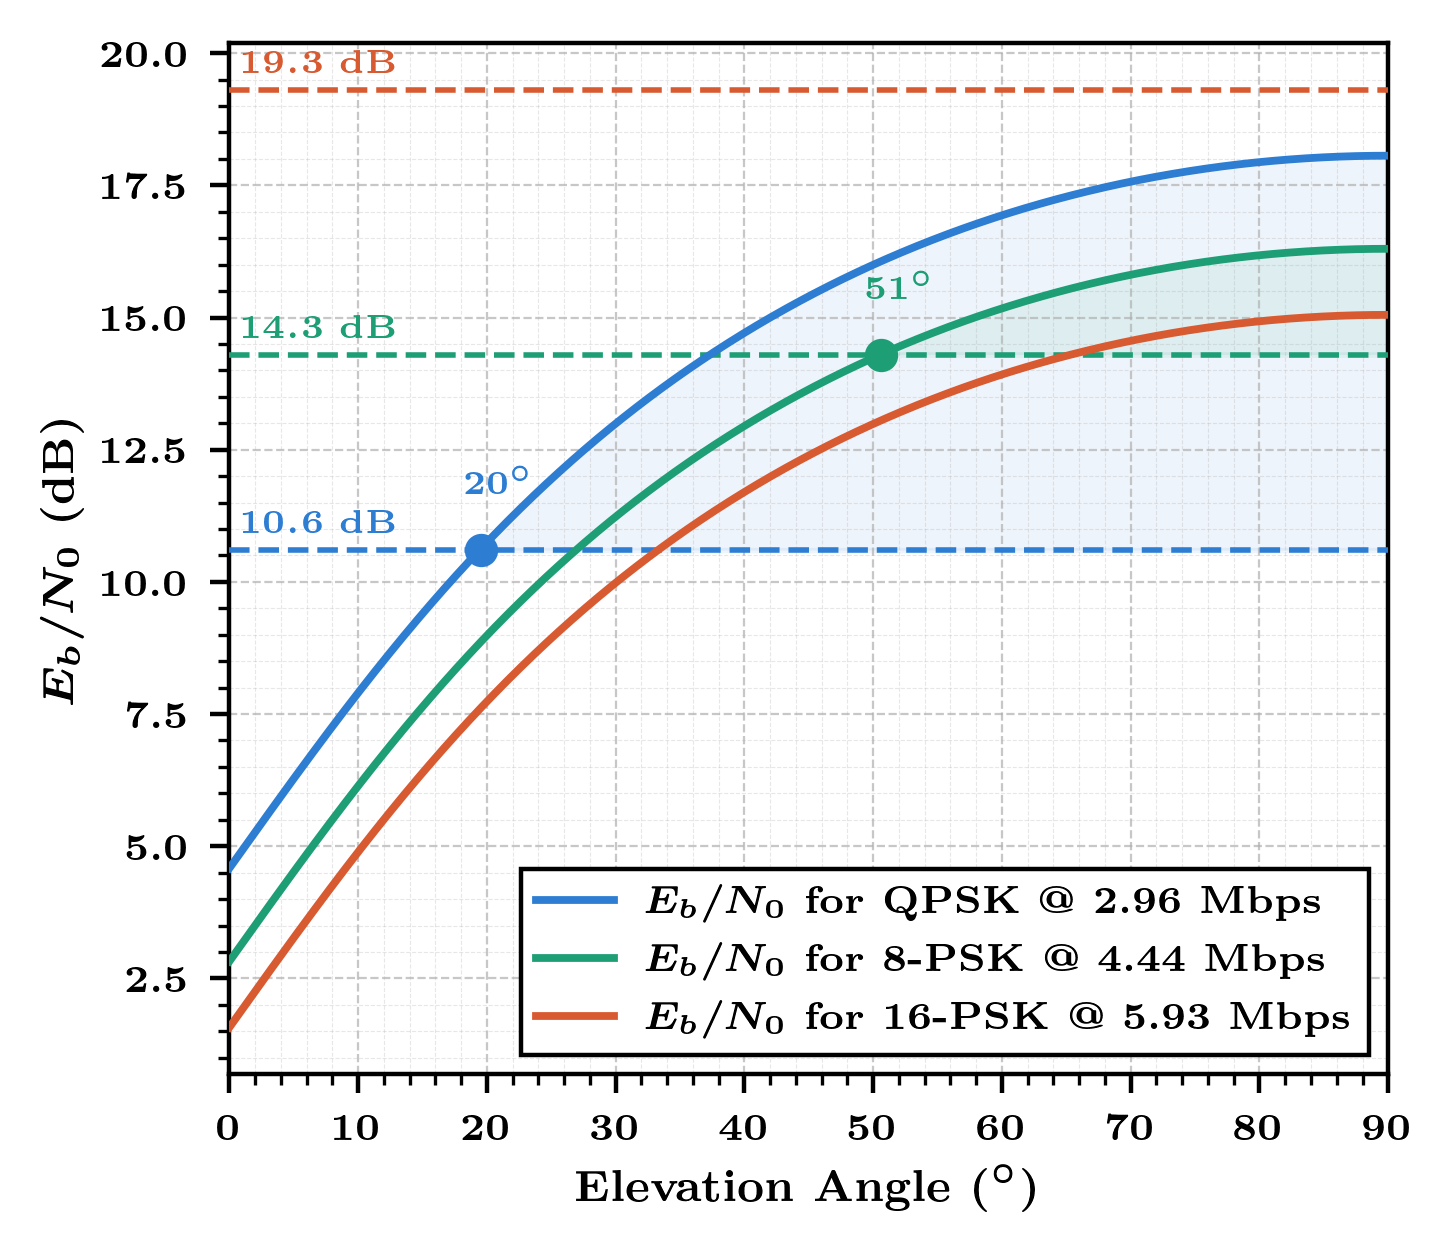
\includegraphics[width=\linewidth]{imgs/link_budget_plot.png}
    \caption{Available $E_b/N_0$ vs. elev. angle for QPSK, 8PSK, and 16PSK over a 2\,MHz BW at 2.2\,GHz. Dashed lines indicate the minimum $E_b/N_0$ required. Filled markers denote the minimum feasible elevation angle for each scheme.}
    \label{fig:link_budget}
\end{figure}

% =========================================================================== %
\subsection{GaN Technology for RF Power Amplifiers}
The demanding requirements of CubeSat RF subsystems, high output power, efficiency, and reliability within tight mass and volume constraints, call for a transistor technology capable of delivering high power density while withstanding the thermal and electrical stresses of space operation. GaN HEMTs have emerged as a strong candidate for this role, and are examined in this section.

GaN is a wide-bandgap semiconductor with a bandgap energy of approximately 3.4\,eV, significantly higher than silicon's 1.12\,eV. This translates into higher breakdown voltages and higher operating temperatures. The higher critical electric field also results in greater electron saturation velocity, which supports operation at microwave and millimeter-wave frequencies \cite{Taur_Ning_2021}.

These transistors are implemented using an AlGaN/GaN heterostructure typically grown on Si, SiC, or sapphire substrates. The lattice mismatch and spontaneous polarization at the AlGaN/GaN interface induce a two-dimensional electron gas (2DEG) with high carrier density and mobility, without doping in the channel region \cite{Ambacher2000}. Most GaN HEMTs, including the device used in this paper, are depletion-mode transistors, meaning the channel conducts by default and a negative gate voltage is required to turn off the device. This characteristic imposes a specific power-up and power-down sequence, the gate bias must be applied before the drain voltage and removed after it, to avoid driving the device into an uncontrolled high-current state that could permanently damage both the transistor and the surrounding circuit. Furthermore, the high power density achievable in GaN devices, with values on the order of 40\,W/mm having been demonstrated \cite{Wu2006}, enables compact implementations well suited to mass and volume-constrained platforms such as CubeSats. The incorporation of field plates at the gate further extends this capability by redistributing the electric field at the gate edge, suppressing peak values and improving both breakdown voltage and linearity \cite{Chiang2012}.

% =========================================================================== %
\subsection{Class AB Operation}
The transistor technology alone does not determine the amplifier's performance, the choice of operating class defines how the device is biased and driven, directly affecting both efficiency and linearity. Class A amplifiers conduct for the full cycle (360\degree), offering the best linearity but a theoretical maximum drain efficiency of only 25\% for a resistive load, a significant limitation for power-constrained platforms such as CubeSats where every milliwatt of dissipated power carries a thermal and energy budget cost. At the opposite extreme, Class C amplifiers conduct for less than half a cycle (below 180\degree), achieving higher theoretical efficiencies but introducing significant nonlinear distortion, incompatible with the constant-envelope modulation schemes discussed in Section~\ref{sec:link_budget}.

Class AB amplifiers conduct for more than half but less than a full cycle. As the conduction angle approaches 180\degree\ (Class B limit), the theoretical drain efficiency approaches 78.5\%, decreasing gradually as the bias is increased toward Class A. This intermediate region allows the designer to balance efficiency, linearity, and device stress within a single topology. Moreover, the power density achievable in GaN devices enables a Class AB design to meet the target output power in a single stage, reducing board area and circuit complexity compared to multi-stage approaches. For CubeSat applications, where both the power budget and signal fidelity are constrained, Class AB provides a practical and robust solution. 

%This choice is consistent with literature on S-Band PAs for satellite and space applications, where Class AB operation has been widely adopted \cite{}. % Otros nombres sugeridos: State of the Art / Related Work
\section{Proposed Approach}
A single-stage Class AB power amplifier was designed to operate at a center frequency of 2.2\,GHz, targeting an output power of 30\,dBm for a drain efficiency of 30\% at the 1\,dB compression point, using the CGH40006S GaN HEMT transistor (MACOM) \cite{Macom}. The circuit was fabricated on a four-layer PCB manufactured by JLCPCB using the JLC04161H-7628 stackup, shown in Table~\ref{tab:pcb_stackup}, which provides a controlled 50\,$\Omega$ impedance for the transmission lines.

\begin{table}[b]
    \caption{PCB Stackup}
    \label{tab:pcb_stackup}
    \centering
    \renewcommand{\arraystretch}{1.1}
    \begin{tabular}{|l|c|c|}
        \hline
        \textbf{Layer} & \textbf{Relative Permittivity (Dk)} & \textbf{Thickness} \\
        \hline
        Top      & \cellcolor{coppercolor}Copper  & 0.035mm   \\ \hline
        Prepreg  & \cellcolor{dielectriccolor}4.4 & 0.21040mm \\ \hline
        Inner L2 & \cellcolor{coppercolor}Copper  & 0.0152mm  \\ \hline
        Core     & \cellcolor{dielectriccolor}4.6 & 1.065mm   \\ \hline
        Inner L3 & \cellcolor{coppercolor}Copper  & 0.0152mm  \\ \hline
        Prepreg  & \cellcolor{dielectriccolor}4.4 & 0.21040mm \\ \hline
        Bottom   & \cellcolor{coppercolor}Copper  & 0.035mm   \\
        \hline
    \end{tabular}
\end{table}

To allow post-fabrication tuning of the transmission lines, additional short traces were included close to other circuit traces throughout the PCB. These traces are unconnected and can be selectively incorporated to introduce stubs of variable length or to extend existing lines, enabling adjustment and further testing of the matching networks without requiring a new board revision. Fig.~\ref{fig:pcb} shows the fabricated PCB.

\begin{figure}[b]
    \centering
    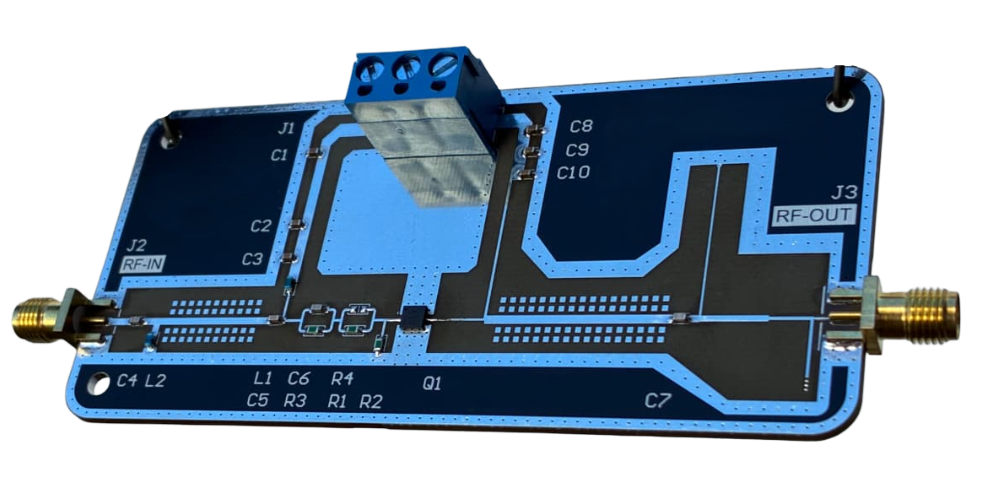
\includegraphics[width=\linewidth]{imgs/placa_sin_logos.png}
    \caption{Fabricated PCB of the proposed 2.2 GHz GaN power amplifier.}
    \label{fig:pcb}
\end{figure}

The overall architecture is shown in Fig.~\ref{fig:pa_diagram}. The input stage comprises a high-pass filter (HPF), a bias-tee, and a stability network, while the output stage consists of a bandpass filter (BPF) and a bias-tee. Both the input and output networks were designed to achieve impedance matching at the operating frequency, with the target impedances determined from load-pull simulation results.

\begin{figure*}[t]
    \centering
    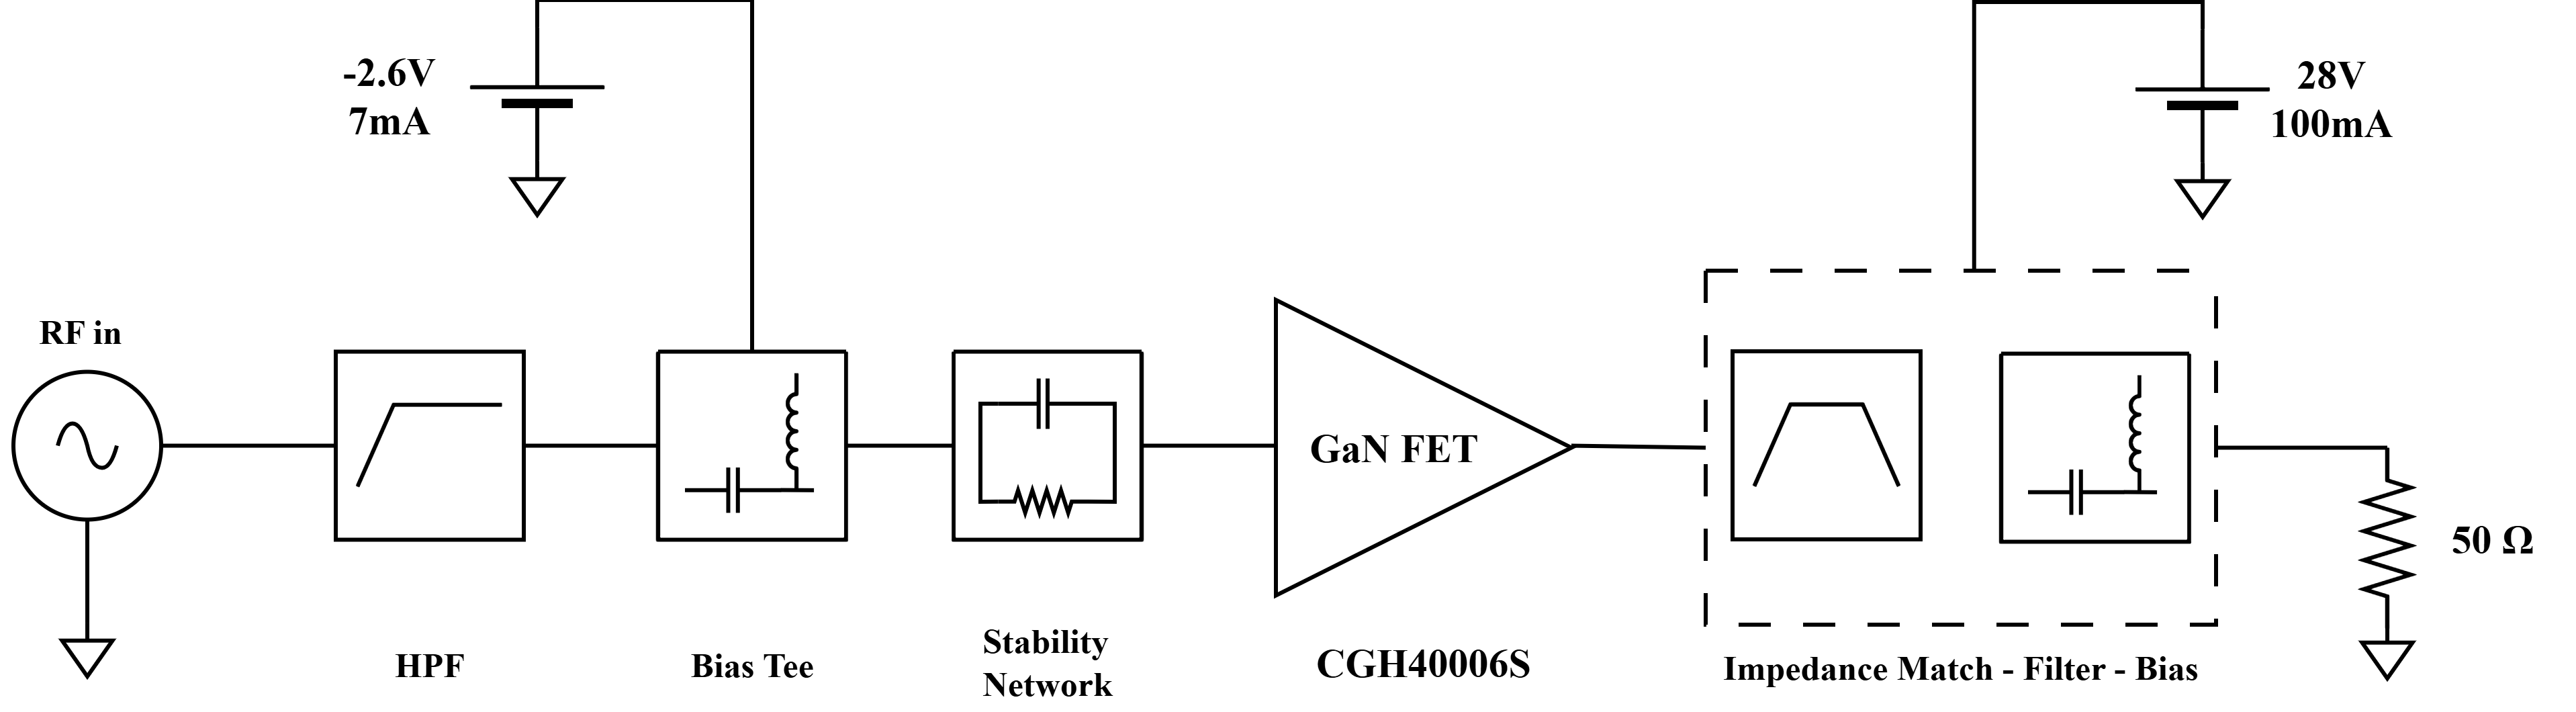
\includegraphics[width=\textwidth]{imgs/pa_block_diagram.png}
    \caption{Block diagram of the proposed power amplifier, including the input matching, biasing, stabilization, and output matching networks.}
    \label{fig:pa_diagram}
\end{figure*}

% =========================================================================== %
\subsection{Circuit Biasing}
Biasing is provided through a bias-tee at each port, consisting of an RF choke and a DC block capacitor. The RF choke presents a high impedance at the operating frequency, isolating the DC supply from the RF signal path, while the DC block capacitor prevents the DC bias from reaching the RF ports. Additional bypass capacitors were placed along the power supply rails to filter out supply noise. The bias point was set at a drain voltage $V_D = 28\,\text{V}$ and a gate voltage $V_G = -2.6\,\text{V}$, resulting in a drain current of $I_D = 100\,\text{mA}$ and a gate bias current of $7\,\text{mA}$, corresponding to Class AB operation.

% =========================================================================== %
\subsection{Simulation-assisted Design Methodology}
The circuit was simulated using a SPICE-based simulator with harmonic balance (HB) analysis. A transistor simulation model and passive component models, including transmission line models, were incorporated. Small-signal S-parameter simulations were used to evaluate the stability of the design over a broad frequency range (0.5–8\,GHz). Load-pull simulation was performed by sweeping input and load impedances under large-signal (HB analysis) conditions to map power-added efficiency (PAE), output power, and gain contours, enabling the selection of the optimal output termination impedance \cite{Cripps2006}.

% =========================================================================== %
\subsection{Load-Pull and Matching Networks}
Load-pull analysis sweeps the load impedance across the Smith chart under large-signal excitation, mapping figures of merit such as PAE, output power, and gain at each impedance point. The resulting contours enable the selection of the termination that best satisfies the target performance trade-off.

The output matching network was designed based on the results of load-pull simulation, which identified the optimal load impedance maximizing PAE at the target output power level. The input matching network was subsequently optimized to maximize power transfer and overall circuit performance. A point offering a favorable trade-off among PAE, gain, and output power was selected from the load-pull contours for an input power of 14 dBm, shown in Fig.~\ref{fig:loadpull_img}. The load-pull analysis determined an optimal load impedance of (24.1 + j52) $\Omega$.

% =========================================================================== %
\subsection{Stability Network}
The small-signal stability of an amplifier can be analyzed by studying the $\mu_{source}$ and $\mu_{load}$ parameters, derived from the S-parameters of the circuit. According to \cite{Edwards1992}, if either parameter exceeds unity for all frequencies, the circuit is unconditionally stable. This constitutes both a necessary and sufficient condition.

Unconditional stability was ensured across the 0.5–8 GHz frequency range by implementing a stabilization network at the transistor gate, consisting of a parallel RC circuit followed by a resistive voltage divider \cite{Bahl2009}. Additionally, a shunt resistor was included on the PCB as an optional post-fabrication tuning element to allow stability adjustments without requiring a board revision. To verify the network's effectiveness, both stability factors were extracted from simulated small-signal S-parameters. As illustrated in Fig.~\ref{fig:stability_img}, $\mu_{source}$ and $\mu_{load}$ exceed unity throughout the entire range, confirming the small-signal unconditional stability of the amplifier.

\begin{figure}
    \centering
    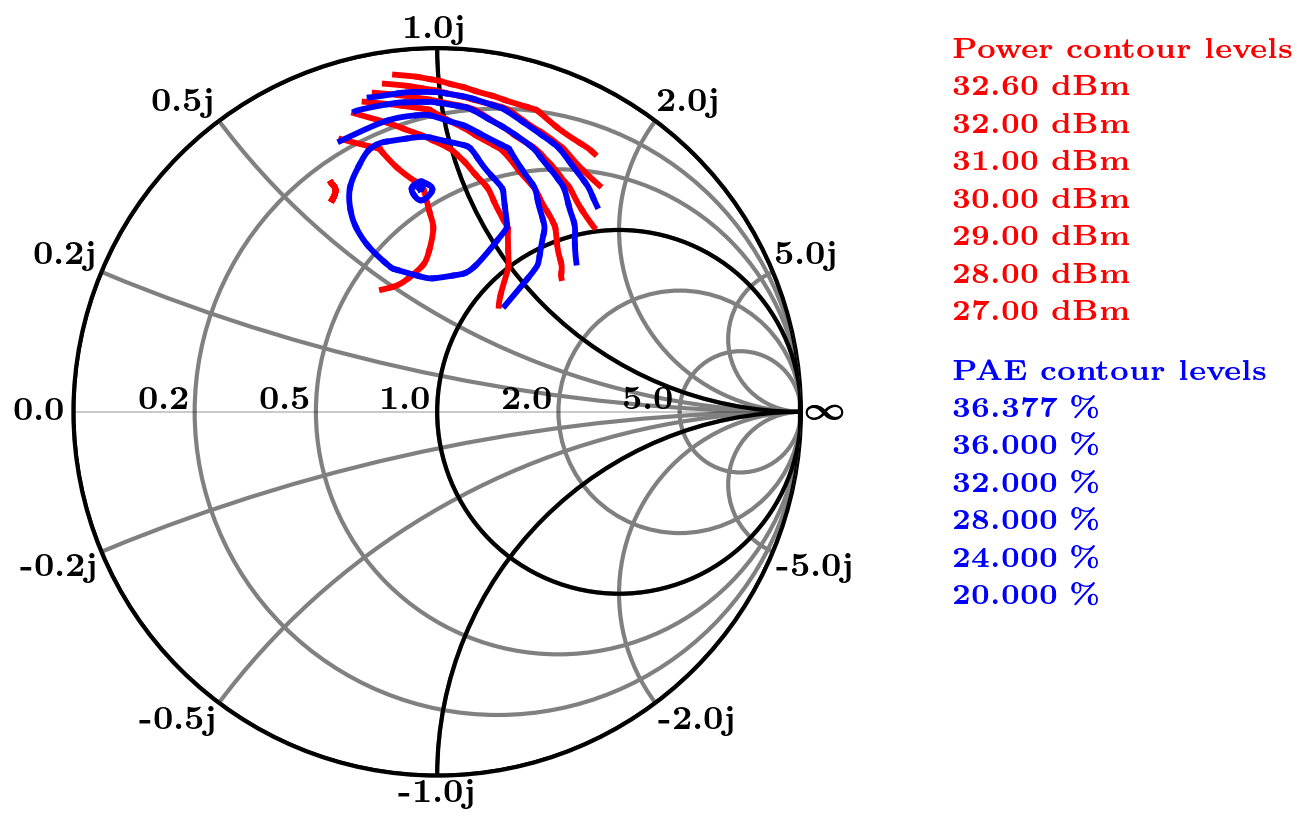
\includegraphics[width=0.48\textwidth]{imgs/load_pull_plot.png}
    \caption{Load-pull simulation contours: PAE (blue) and $P_{out}$ (red) on the Smith chart}
    \label{fig:loadpull_img}
    
    \vspace{0.5em}
    
    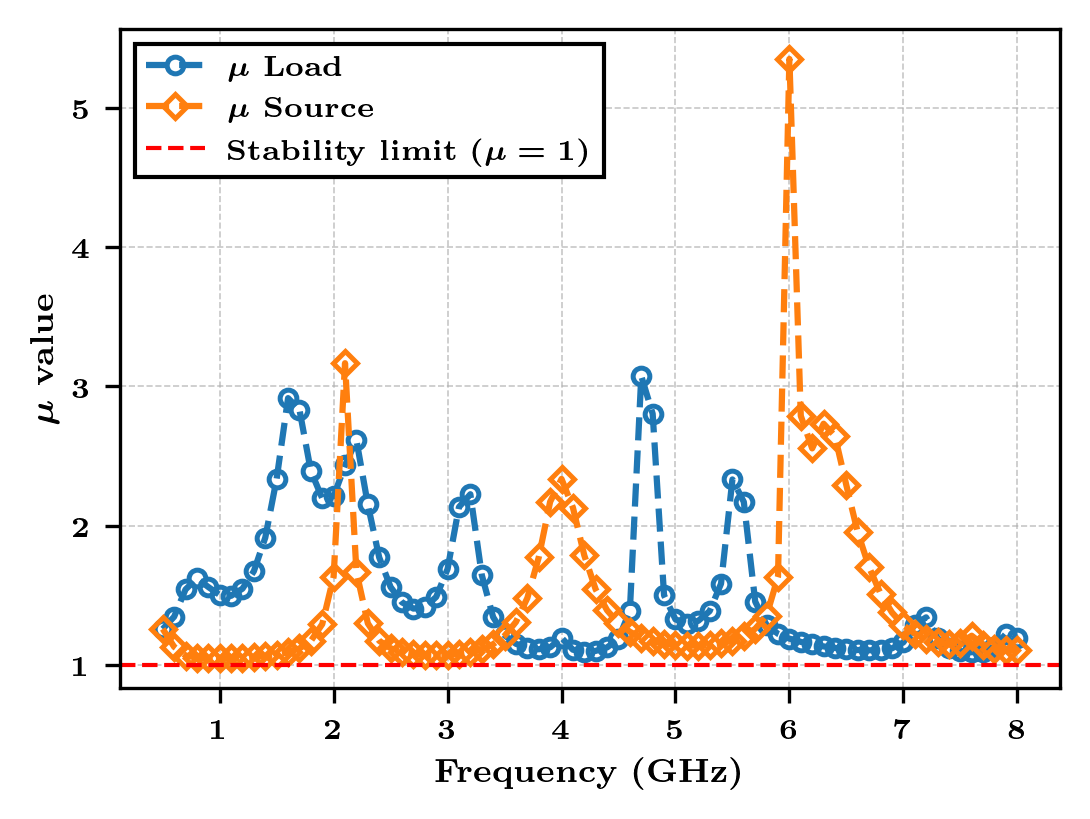
\includegraphics[width=0.48\textwidth]{imgs/stability_plot.png}
    \caption{Simulated source and load stability factors ($\mu$) as a function of frequency. The load stability factor (blue) and source stability factor (orange) remain above the unconditional stability threshold ($\mu=1$, red dashed line) across the whole frequency range, indicating stable operation.}
    \label{fig:stability_img}
\end{figure}

% =========================================================================== %
\subsection{Output Waveforms}
A 5th-order harmonic balance simulation was conducted to analyze the large-signal spectral response of the proposed design and evaluate the harmonic content at the output, providing insight into the nonlinear behavior of the amplifier under operating conditions. The input RF power was set to 14\,dBm into a 50\,$\Omega$ matched load. Fig.~\ref{fig:spectrum} shows the simulated output harmonic spectrum from the fundamental frequency up to the fifth harmonic.

\begin{figure}[t]
    \centering
    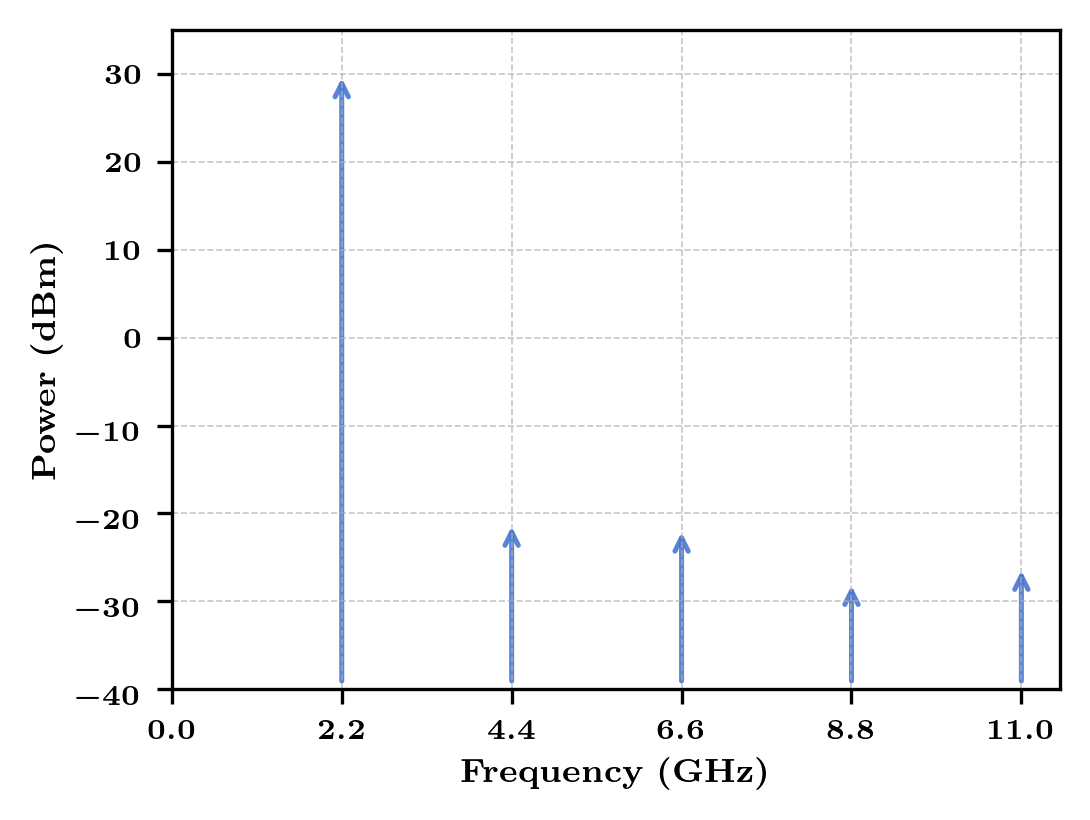
\includegraphics[width=\linewidth]{imgs/spectrum_plot.png}
    \caption{Harmonic balance simulation results showing the output power spectrum up to the fifth harmonic.}
    \label{fig:spectrum}
\end{figure}
\section{Measurement Setups}
To experimentally validate the design, a set of measurements was carried out covering small-signal behavior, large-signal power performance, and nonlinear characterization. Each measurement required a dedicated setup, described in the following subsections.

% =========================================================================== %
\subsection{S-Parameters Measurement Setup}
S-parameters were measured to validate the matching network design and characterize the small-signal behavior of the amplifier. A Keysight N5242B PNA-X vector network analyzer (VNA), calibrated using the TOSM method with a Keysight 85052B calibration kit, was employed. A fixed 30\,dB attenuator was inserted at the output port to protect the VNA receiver from high power levels. Consequently, only $S_{21}$ and $S_{11}$ are reported. The attenuator's effect was de-embedded from the measured $S_{21}$ by adding the nominal attenuator value.

% =========================================================================== %
\subsection{Power Output Measurement Setup}
A power output measurement was carried out to characterize the large-signal behavior of the amplifier. Since the device under test requires drive levels beyond the native output capability of the measurement instrument, a Mini-Circuits ZX60-83LN12+ driver amplifier was inserted between the Keysight N5242B signal source and the PA under test. Output power was measured with a Keysight U8485A power sensor preceded by a 20\,dB attenuator and a 10\,dB attenuator, as shown in Fig.~\ref{fig:power_meas_setup}. The input was swept in 2.5\,dBm steps at the nominal operating frequency of 2.2\,GHz. The values obtained from this measurement were used to determine the gain and the 1\,dB compression point of the amplifier.

\begin{figure}[b]
    \centering
    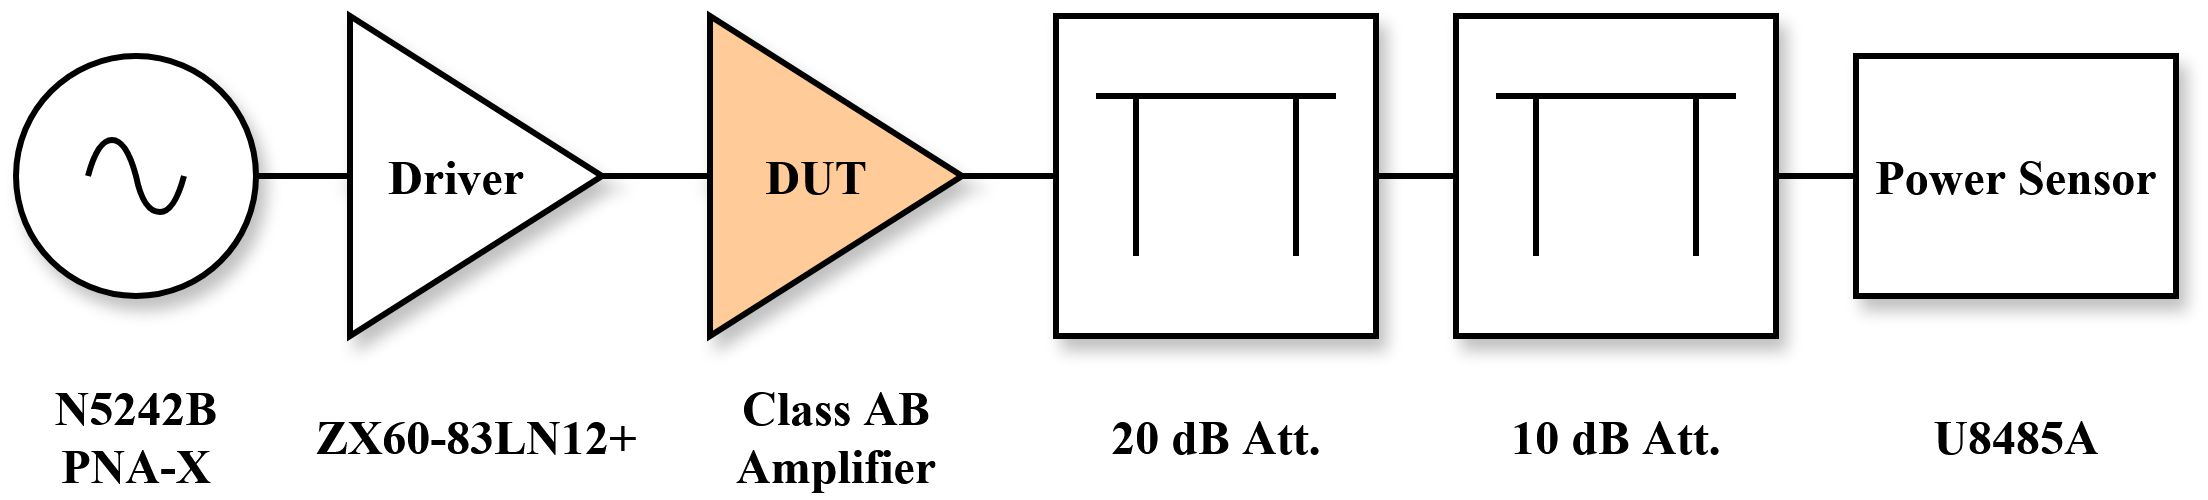
\includegraphics[width=0.48\textwidth]{imgs/p1db_blocks.png}
    \caption{Output power measurement setup including the PNA as RF signal source, driver amplifier, DUT, two cascaded attenuators at the DUT output, and a power sensor.}
    \label{fig:power_meas_setup}
\end{figure}

% =========================================================================== %
\subsection{Harmonic Power Measurement Setup}
Due to the intrinsic nonlinearity of any active device, as well as the operating class at which the amplifier is biased, PAs generate harmonic distortion that degrades spectral purity and may cause out-of-band interference. To characterize this behavior, the second and third harmonics were measured using a Siglent SSG3032X-IQE signal generator as the CW RF source at 2.2\,GHz and a Keysight N9322C spectrum analyzer at the output, as illustrated in Fig.~\ref{fig:hb_setup}. A 20\,dB attenuator was placed at the analyzer input for protection. The input power was swept from 0\,dBm to 20\,dBm in 5\,dBm steps.

\begin{figure}[t]
    \centering
    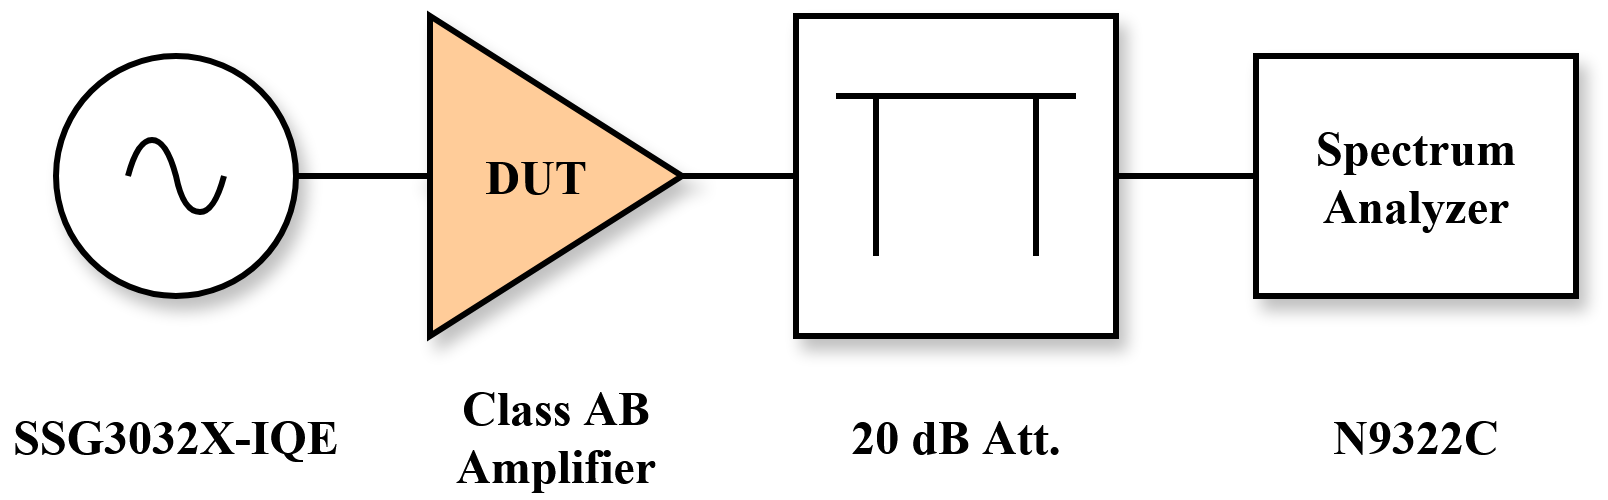
\includegraphics[width=0.48\textwidth]{imgs/harmonic_balance_blocks.png}
    \caption{Harmonic power measurement setup including the RF signal source, DUT, the 20 dB attenuator, and the spectrum analyzer.}
    \label{fig:hb_setup}
\end{figure}

% =========================================================================== %
\subsection{OIP3 Measurement Setup}
The third-order intercept point (OIP3) was obtained using the "IMD Sweep"(S93087B IMD) software application of the Keysight N5242B PNA-X VNA \cite{KeysightPNAConfig}. As with the power output measurement, a Mini-Circuits ZX60-83LN12+ driver amplifier was added between the VNA's signal source and the DUT to reach the drive levels required to manifest the amplifier's nonlinear effects. Also, two attenuators of 20\,dB and 10\,dB were added to the DUT output to protect the VNA ports.

The frequency separation of the tones was set to 10 MHz, and their power was set to $P_{in} = -5 \,\text{dBm}$ 

\section{Experiments and Results}
\subsection{Measured S-Parameters}
Figs.~\ref{fig:s11_plot} and~\ref{fig:s21_plot} present the simulated and measured $S_{11}$ and $S_{21}$ parameters, respectively, over the DC--5\,GHz range. A resonance outside the band of interest was identified in the measured response. This feature was not predicted by the original simulation model and is attributed to parasitic effects of the PCB layout and component packaging that were not fully captured in the initial model.

The measured center frequency is 2.11\,GHz, corresponding to a 90\,MHz shift from the design target of 2.2\,GHz. This shift is attributed to the series equivalent inductance (ESL) of the stabilization resistors, which was not accounted for in the original model. Incorporating an ESL of 0.5\,nH per resistor, a value consistent with published data for 0603-package thin-film resistors \cite{VishayTN}, brings the simulated center frequency into agreement with the measurement. The overall small-signal behavior closely matches the design objectives.

\begin{figure*}[t]
    \centering
    \begin{minipage}{0.48\textwidth}
        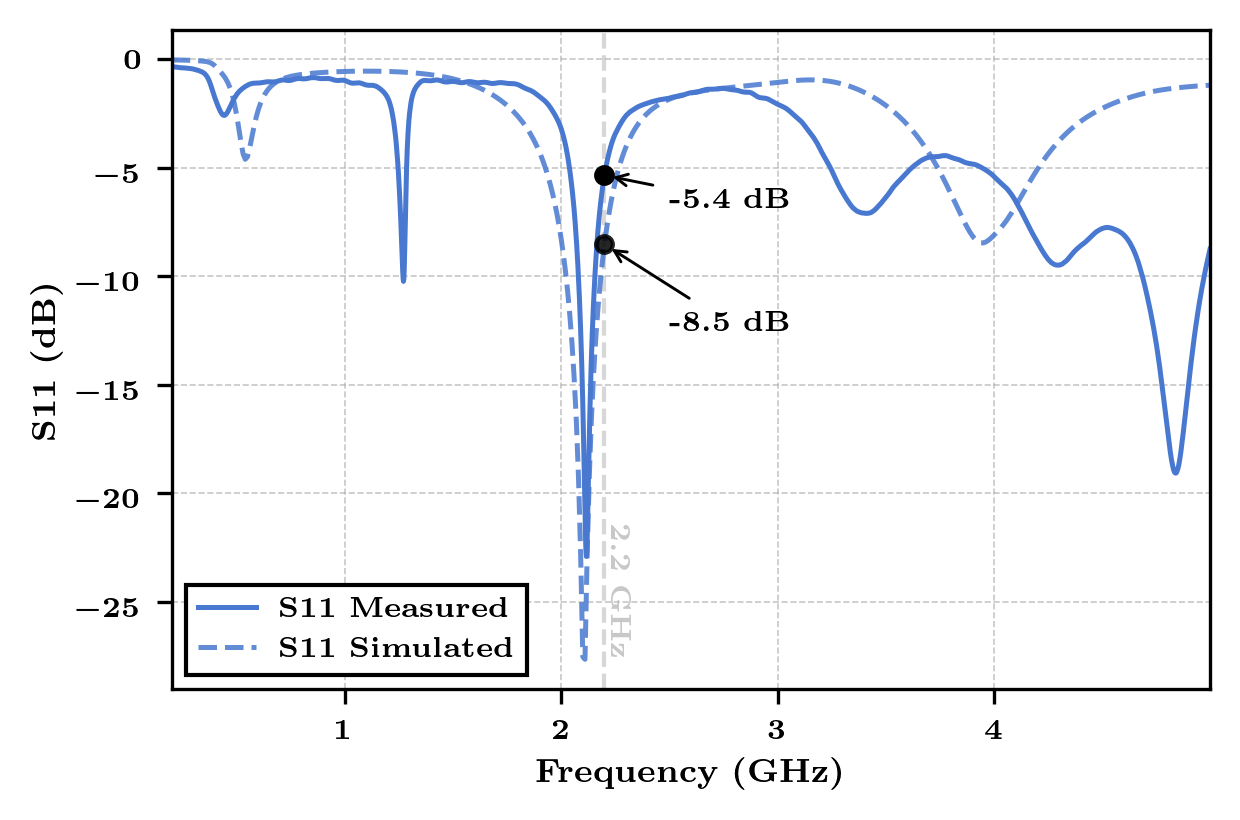
\includegraphics[width=\linewidth]{imgs/s11_plot.png}
        \caption{Comparison of the simulated (dashed line) and measured (solid line) $S_{11}$ of the fabricated power amplifier.}
        \label{fig:s11_plot}
    \end{minipage}
    \hfill
    \begin{minipage}{0.48\textwidth}
        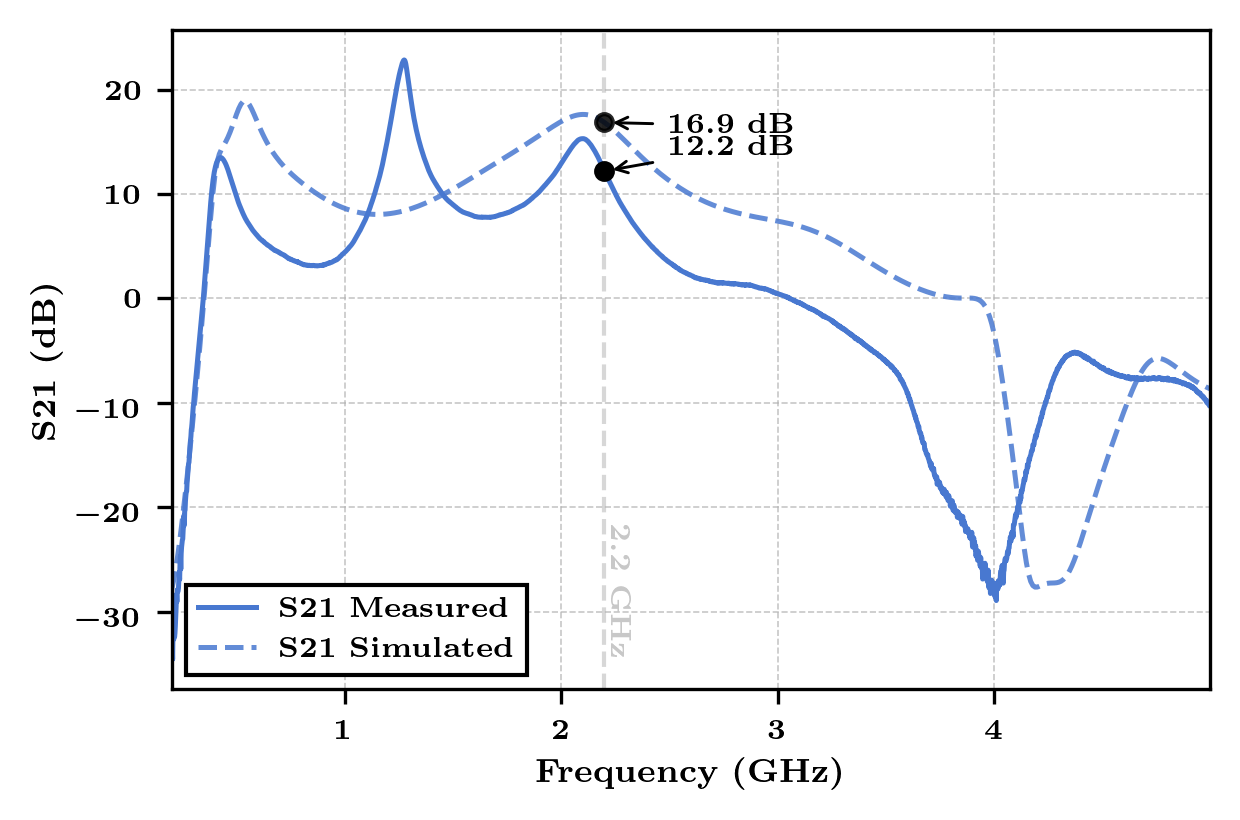
\includegraphics[width=\linewidth]{imgs/s21_plot.png}
        \caption{Comparison of the simulated (dashed line) and measured (solid line) $S_{21}$ of the fabricated power amplifier.}
        \label{fig:s21_plot}
    \end{minipage}
\end{figure*}

% =========================================================================== %
\subsection{P1dB Extraction}
The 1\,dB gain compression point (P1dB) is a key figure of merit for power amplifiers, defined as the input power level at which the output power deviates by 1\,dB from the extrapolated small-signal linear response. It marks the boundary of the amplifier's linear operating region \cite[pp.~512--513]{Pozar2012}.

Fig.~\ref{fig:p1db_img} shows the measured output power as a function of input power for the complete test chain (driver amplifier and PA under test). Because the driver amplifier itself enters compression within the measurement range, the P1dB of the system under test cannot be read directly from the measured output power curve. Instead, the cascade compression expression~\eqref{eq_p1db} was applied, which refers the compression of each stage to the system input and combines their contributions inversely weighted by the gain of the preceding stages~\cite{Dong2021}. The PA P1dB was extracted by solving this expression using the known gain and compression values of the driver stage, yielding a P1dB of 30.3\,dBm at an operating frequency of 2.2\,GHz.

\begin{equation}
    \scalebox{0.85}{$\displaystyle 
        \frac{1}{P_{1dB_{sys}}} = \frac{1}{G_2\cdots G_N P_{1dB_1}} + \frac{1}{G_3\cdots G_N P_{1dB_2}} + \cdots + \frac{1}{P_{1dB_N}}$
    }
    \label{eq_p1db}
\end{equation}

\begin{figure}[t!]
    \centering
    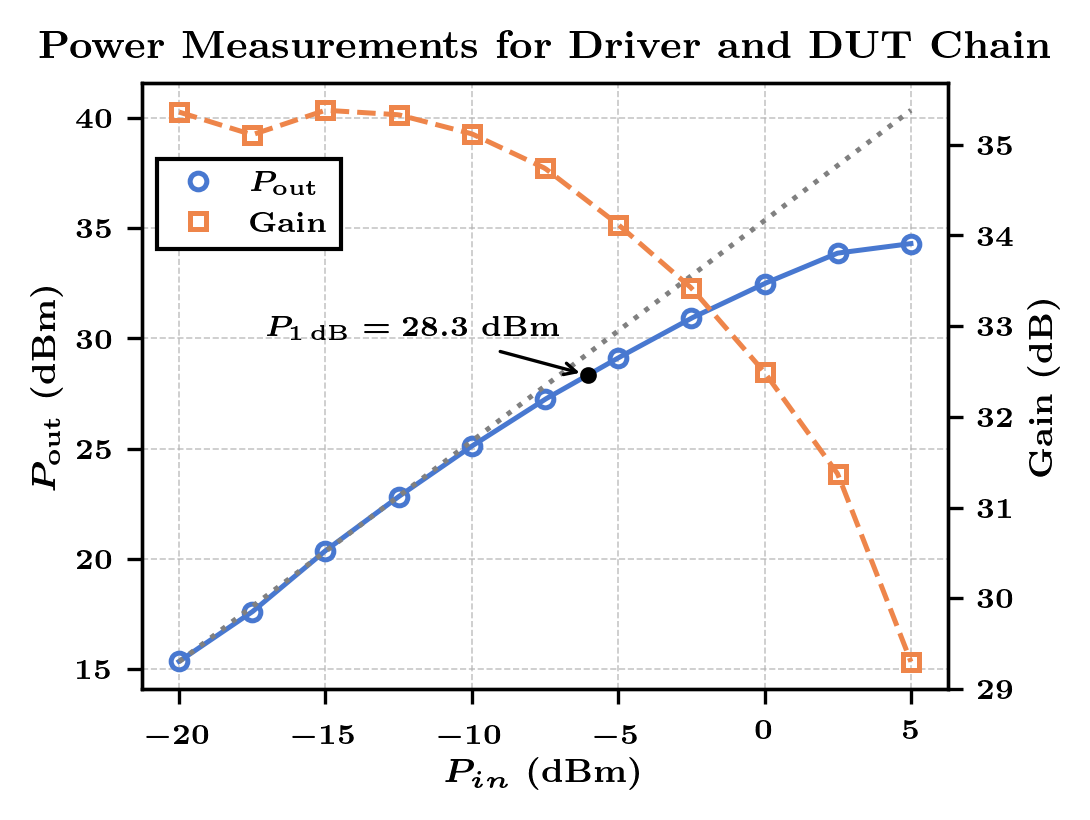
\includegraphics[width=0.48\textwidth]{imgs/p1db_plot.png}
    \caption{Measured output power (blue) and gain (orange) as a function of input power for the driver-DUT chain. The dotted gray line represents the ideal linear transfer characteristic obtained from the small-signal gain extrapolation.}
    \label{fig:p1db_img}
\end{figure}

% =========================================================================== %
\subsection{Gain, Drain efficiency and Bandwidth}
\subsubsection{Gain}
The small-signal gain of the amplifier was extracted from the power measurement chain. The input and output power at the PA terminals were computed as:

\begin{align}
    P_{in,PA}  &= P_{in,sys} + G_{driver} \label{eq_pin} \\
    P_{out,PA} &= P_{out,sys} + |A_{att}| \label{eq_pout}
\end{align}

where $P_{in,sys}$ is the system input power, $G_{driver}$ is the gain of the driver stage, $P_{out,sys}$ is the measured system output power, and $|A_{att}|$ is the total attenuation of the attenuator chain, with all quantities in dBm and dB respectively. The gain was then calculated as:

\begin{equation}
    G = P_{out,PA} - P_{in,PA}
    \label{eq_gain}
\end{equation}

A small-signal gain of 13.26\,dB was obtained.

% =========================================================================== %
\subsubsection{Drain Efficiency}
Drain efficiency ($\eta_D$) was evaluated at the measurement point closest to the 1\,dB compression point, corresponding to an output power of 30.92\,dBm, and computed as:

\begin{equation}
    \eta_D = \frac{P_{out,PA}}{P_{DC}} \times 100\%
    \label{eq_eta}
\end{equation}

where $P_{out,PA}$ is the output power delivered by the amplifier and $P_{DC}$
is the DC power consumed. A drain efficiency of 32.94\% was obtained. The power-added efficiency at the same operating point, computed as

\begin{equation}
    \text{PAE} = \frac{P_{out,PA} - P_{in,PA}}{P_{DC}} \times 100\%,
    \label{eq_pae}
\end{equation}

was 30.51\%.

\subsubsection{Bandwidth}
The operating bandwidth was determined from the measured $S_{11}$ response. The two frequency points at which $S_{11}$ crosses the $-10$\,dB threshold within the region of interest were identified, and the bandwidth was defined as their difference, obtaining a 70\,MHz value.

% =========================================================================== %
\subsection{Measured Harmonic Distortion}
The second and third harmonics were measured at $P_{in}=20\,\text{dBm}$, approximately at the P1dB operating point, representing the worst-case nonlinear condition during normal amplifier operation. The second harmonic rejection was 26.74 dBc and the third harmonic rejection was 42.21 dBc. These values represent the minimum expected performance in linear operation below P1dB. The measured harmonic content differs from the simulation model, which is attributed to a frequency shift in the output filter's rejection band. This can be observed in the amplifier's forward transmission response (S21), where the output filter stopband appears shifted toward lower frequencies.


% =========================================================================== %
\subsection{Measured OIP3}
The output-referred third-order intercept point (OIP3) is another parameter that characterizes the nonlinear behavior of the amplifier. It is a figure of merit that indicates the output power at which the third-order intermodulation products (IM3) become comparable to the fundamental signal. It is an important value as the IM3s are typically encountered in the operating band. The OIP3 is a theoretical point defined as the intersection of the extrapolation of the output power transfer curve with respect to the input power, with a unity slope on a log-log scale, and the extrapolation of the IM3 response as a function of the input power, where the slope is 3 dB/dB for the same scale ~\cite[pp.~515--517]{Pozar2012}.

The OIP3 was determined for the driver and power amplifier chain. Fig.~\ref{fig:oip3} shows the OIP3 of the chain for a wide range of frequencies. As with the P1dB, the nonlinearity of the driver amplifier affects the chain OIP3. For this reason, the OIP3 value for the DUT was obtained from equation ~\eqref{eq_oip3}.

\begin{equation}
    \scalebox{0.85}{$\displaystyle 
        OIP3_{sys} = \left(\frac{1}{OIP3_{N-1} \cdot G_N} + \frac{1}{OIP3_N}\right)^{-1}$
    }
    \label{eq_oip3}
\end{equation}

An OIP3 of $39.83\,\text{dBm}$ was obtained. This value is consistent with the expected experimental relationship between the P1dB and the OIP3, where the OIP3 is usually 10 to 15 dB larger than the P1dB~\cite[p.~516]{Pozar2012}.

\begin{figure}[b]
    \centering
    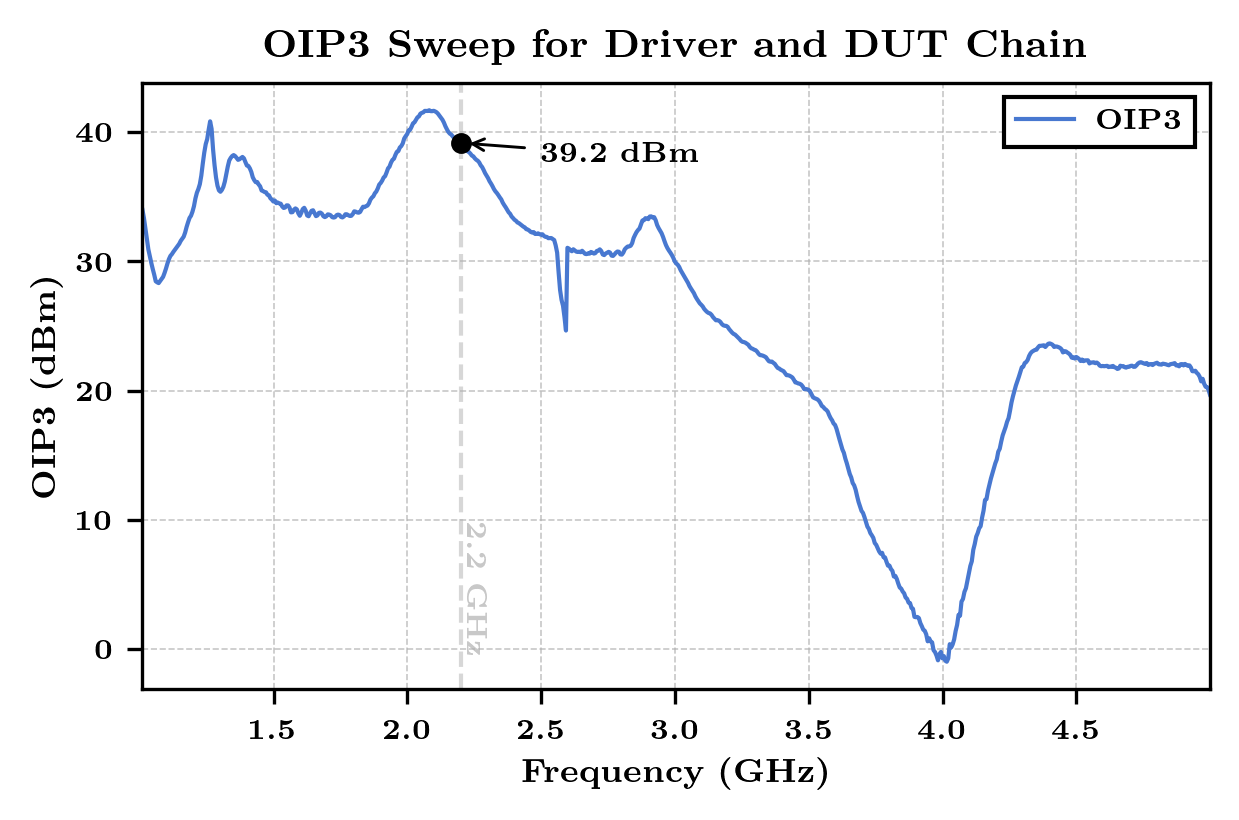
\includegraphics[width=1\linewidth]{imgs/oip3_plot.png}
    \caption{Frequency sweep of the measured output third-order intercept point (OIP3) for the driver–DUT chain.}
    \label{fig:oip3}
\end{figure}


% =========================================================================== %
\subsection{Summary of Results}
Table~\ref{tab:pa_results} summarizes the key measured performance parameters of the fabricated amplifier, providing a consolidated overview of the characterization results presented throughout this section.

\begin{table}[ht]
    \caption{RF Power Amplifier Measured Performance Summary}
    \label{tab:pa_results}
    \centering
    \renewcommand{\arraystretch}{1.15}
        \begin{tabular}{lc}
        \hline\hline
        \textbf{Parameter}                         & \textbf{Value}                 \\
        \hline
        Center Frequency                           & 2.11\,GHz                      \\
        Bandwidth (BW)                             & 70\,MHz                        \\
        1\,dB Compression Point ($P_{1\text{dB}}$) & 30.30\,dBm                     \\
        Third-Order Intercept ($\text{OIP}_3$)     & 39.83\,dBm                     \\
        Small-Signal Gain                          & 13.26\,dB                      \\
        Drain Efficiency                           & 32.94\% @ $P_{out}=30.92$\,dBm \\
        PAE                                        & 30.51\% @ $P_{out}=30.92$\,dBm \\
        VSWR                                       & $<$1.92:1                      \\
        \hline\hline
        \end{tabular}
\end{table}
\section{Conclusions}
An S-band power amplifier was designed, fabricated and characterized. The experimental results are aligned with the design requirements. A favorable compromise was obtained between output power and linearity, with a P1dB of 30.3 dBm and an OIP3 of 39.83 dBm. The drain efficiency reached 32.94\% at an output power of 30.9 dBm. The design parameters are summarized in Table~\ref{tab:pa_results}.

The obtained output power and bandwidth validate the module for data transmission at a 2.96 Mbps rate with a BER lower than $10^{-5}$ for the downlink in LEO missions.

Finally, the correlation between experimental results and simulated values confirms the proposed design methodology, consolidating a development and characterization platform for RF modules that can be reused in future aerospace applications.
%\lipsum[5-9]

% ========================= ACKNOWLEDGMENT =========================
\section*{Acknowledgment}
\begin{comment}
\textbf{[TODO: REDACTAR AGRADECIMIENTOS]}
Gracias Gabriel Sanca, Marcelo Doallo, UNSAM, CNEA.    
\end{comment}

% ========================= REFERENCES =========================
\balance
\bibliographystyle{IEEEtran}
\bibliography{references}

%\nocite{*}

\end{document}

% Avoid the stilted expression ``one of us (R. B. G.) thanks $\ldots$''. 
% Instead, try ``R. B. G. thanks$\ldots$''. 
% Put sponsor acknowledgments in the unnumbered footnote on the %first page.

%\section*{References}
%The sentence punctuation follows the bracket \cite{b2}. 
%Refer simply to the reference number, as in \cite{b3}---do not use ``Ref. \cite{b3}'' or ``reference 
%\cite{b3}'' except at the beginning of a sentence: ``Reference \cite{b3} was the first $\ldots$''

%Number footnotes separately in superscripts. 
%Place the actual footnote at the bottom of the column in which it was cited. 
%Do not put footnotes in the abstract or reference list. Use letters for table footnotes.

%Capitalize only the first word in a paper title, except for proper nouns and  element symbols.